%---------------------------------------------------------------------------
%	Document Class
%---------------------------------------------------------------------------
\documentclass{Classes/solutionclass} 
%---------------------------------------------------------------------------
%	Header and Footer Styling
%---------------------------------------------------------------------------
\pagestyle{fancy}
\fancyhead[L]{\footnotesize{Taylor Larrechea}}
\fancyfoot[L]{\footnotesize{CSPB 2820}}
\fancyhead[C]{\footnotesize{Linear Algebra With Computer Science Applications}}
\fancyhead[R]{\footnotesize{University of Colorado}}
\fancyfoot[R]{\footnotesize{Study Guide 3 - Norm And Distance}}
\backgroundsetup{
    scale = 1,
    angle = 0,
    opacity = 0.1,
    contents = {
    
\includegraphics[scale = 0.25, keepaspectratio]{Figures/CU Seal.png}
    }
}
%---------------------------------------------------------------------------
%	Begin Document
%---------------------------------------------------------------------------
\begin{document}
% ------------------------- Front Page Info
\pretitle
{CSPB 2820}
{\normalsize{Linear Algebra With Computer Science Applications}}
{\normalsize{Study Guide 3 - Norm And Distance}}
{Taylor Larrechea}
%---------------------------------------------------------------------------
%	Sections
%---------------------------------------------------------------------------
% ------------------------- Sections Table
\makeatletter
    \startcontents[sections]
    \thispagestyle{fancy}
\makeatother
\vspace{-2em}
%---------------------------------------------------------------------------
%	Introduction / Individual Sections
%---------------------------------------------------------------------------
% % ------------------------- Assignment
\clearpage
\chapter{Study Guide 3}

\section{Norm And Distance}
\horizontalline{0}{0}

\begin{center}
    \large{\textbf{Study Guide Instructions}}
\end{center}

\horizontalline{-1}{0}

\begin{itemize}
    \item Submit your work in Gradescope as a PDF - you will identify where your “questions are.”
    \item Identify the question number as you submit.  Since we grade "blind" if the questions are NOT identified, the work WILL NOT BE GRADED and a 0 will be recorded. Always leave enough time to 
    identify the questions when submitting.
    \item One section per page (if a page or less) - We prefer to grade the main solution in a single page, extra work can be included on the following page.
    \item Long instructions may be removed to fit on a single page.
    \item \textbf{Do not start a new question in the middle of a page.}
    \item Solutions to book questions are provided for reference.
    \item You may NOT submit given solutions - this includes minor modifications - as your own.
    \item Solutions that do not show individual engagement with the solutions will be marked as no credit and can be considered a violation of honor code.
    \item If you use the given solutions you must reference or explain how you used them, in particular...
\end{itemize}

\horizontalline{-1}{0}

\begin{center}
    \large{\textbf{Method Selection}}
\end{center}

\horizontalline{-1}{0}

\textbf{For full credit,  EACH book exercise in the Study Guides must use one or more of the following methods and FOR EACH QUESTION.  Identify the number the method by number to ensure full credit.}

\begin{itemize}
    \item \textbf{Method 1} - Provide original examples which demonstrate the ideas of the exercise in addition to your solution.
    \item \textbf{Method 2} - Include and discuss the specific topics needed from the chapter and how they relate to the question.
    \item \textbf{Method 3} - Include original Python code, of reasonable length (as screenshot or text)  to show how the topic or concept was explored.
    \item \textbf{Method 4} - Expand the given solution in a significant way, with additional steps and comments. All steps are justified. This is a good method for a proof for which you are only given a basic outline.
    \item \textbf{Method 5} - Attempt the exercise without looking at the solution and then the solution is used to check work. Words are used to describe the results.
    \item \textbf{Method 6} - Provide an analysis of the strategies used to understand the exercise, describing in detail what was challenging, who helped you or what resources were used. The process of understanding is
    described.
\end{itemize}

% Problem 1
\begin{problem}{Problem 1}
    \begin{statement}{Problem Statement}
        Select one page or section of Chapter Three of VMLS to annotate. Include a screenshot of your annotation here.
    \end{statement}

    For Chapter Three of VMLS, I am annotating \textbf{page 57} of VMLS. The annotations for this problem can be seen on the following page.

    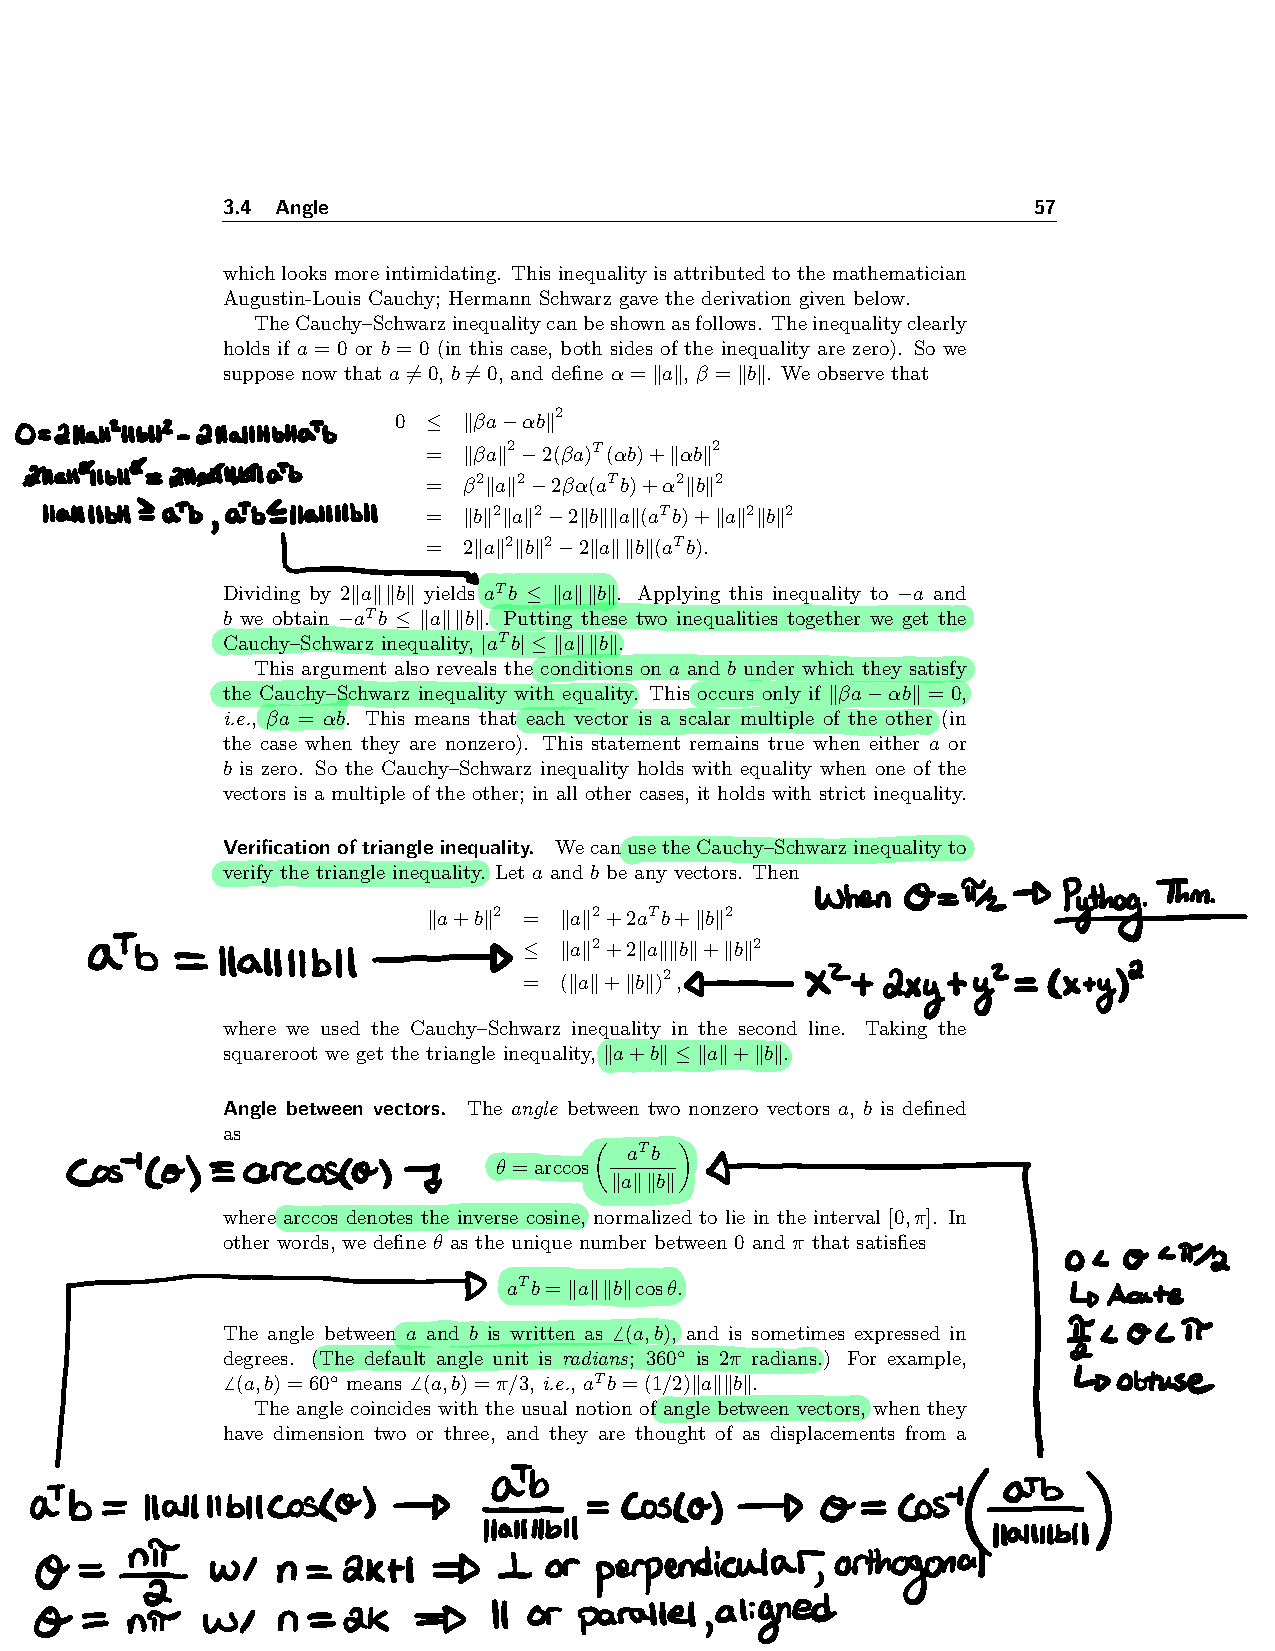
\includepdf[pages={-}, pagecommand={\thispagestyle{fancy}}, width=\paperwidth, offset=0 0]{./PDF/Annotations.pdf}
\end{problem}

% Problem 1 Summary
\begin{summary}{Problem 1 Summary}
    \begin{statement}{Procedure}
        \begin{itemize}
            \item Annotate a page of the textbook and highlight the important aspects from the page
        \end{itemize}
    \end{statement}
    \begin{statement}{Key Concepts}
        \begin{itemize}
            \item This page encapsulates important aspects of the Triangle Inequality
            \item This page also encapsulates how to calculate the angle between two vectors
        \end{itemize}
    \end{statement}
    \begin{statement}{Variations}
        \begin{itemize}
            \item We could be asked to annotate a different section or page of the textbook
        \end{itemize}
    \end{statement}
\end{summary}

% Problem 2
\begin{problem}{Problem 2}
    \begin{statement}{Problem Statement}
        Solve the Chapter 3 Random exercise from the video and Piazza in your own words here. \vspace*{1em}

        \textbf{Original Question:} \vspace*{1em}

        \textit{Norm of sum.} Use formulas (3.1) and (3.6) to show the following:

        \begin{enumerate}[label=(\alph*)]
            \item $a \perp b$ if and only if $||a+b|| = \sqrt{||a||^{2} + ||b||^{2}}$.
            \item Nonzero vectors $a$ and $b$ make an acute angle if and only if $||a + b|| > \sqrt{||a||^{2} + ||b||^{2}}$.
            \item Nonzero vectors $a$ and $b$ make an obtuse angle if and only if $||a + b|| < \sqrt{||a||^{2} + ||b||^{2}}$.
        \end{enumerate}
        Draw a picture illustrating each case in 2-D.
    \end{statement}

    \begin{highlight}[Solution - Part (a)]
        For this problem I will be using \textbf{Method 4}. \vspace*{1em}

        Equation (3.1) from VMLS states that for two vectors $a$ and $b$

        \setcounter{equation}{0}
        \begin{equation}
            ||a + b|| = \sqrt{||a||^{2} + 2a^{T}b + ||b||^{2}}.
        \end{equation}

        Equation (3.6) from VMLS states that for two vectors $a$ and $b$

        \begin{equation}
            ||a + b||^{2} = ||a||^{2} + 2||a||||b||\cos{(\theta)} + ||b||^2.
        \end{equation}

        Taking the square root on each side of equation (2) we have

        \begin{equation}
            ||a + b|| = \sqrt{||a||^{2} + 2||a||||b||\cos{(\theta)} + ||b||^2}.
        \end{equation}

        Two vectors are said to be orthogonal if the angle ($\theta$) between them is $n (90)^{\circ}$ or $\frac{n\pi}{2}$ radians with $n = 2k + 1$. Graphically this is can be seen below

        \begin{center}
            \begin{tikzpicture}
                \draw[->,thick] (0,0)--(2,0) node[right]{$+x$};
                \draw[->,thick] (0,0)--(0,2) node[above]{$+y$};
                \draw[->,blue] (0,0)--(1,0) node[anchor=north west]{$\mathbf{a}$};
                \draw[->,red] (0,0)--(0,1) node[anchor=south east]{$\mathbf{b}$};
                \draw (0.3,0) arc (0:90:0.3);
                \node at (0.4,0.4) {$\theta$};
            \end{tikzpicture}
            \hspace*{10pt}
            \begin{tikzpicture}
                \draw[->,thick] (0,0)--(2,0) node[right]{$+x$};
                \draw[->,thick] (0,0)--(0,-2) node[below]{$-y$};
                \draw[->,blue] (0,0)--(1,0) node[anchor=north west]{$\mathbf{a}$};
                \draw[->,red] (0,0)--(0,-1) node[anchor=south east]{$\mathbf{b}$};
                \draw (0.3,0) arc (0:270:0.3);
                \node at (-0.4,0.4) {$\theta$};
            \end{tikzpicture}
        \end{center}

        In the above image, we see that the angle between these two vectors is $\frac{n\pi}{2}$ radians with $n = 2k + 1$. If we insert this angle into equation (3) we then see that

        \begin{align}
            ||a + b|| & = \sqrt{||a||^{2} + 2||a||||b||\cos{(n\pi / 2)} + ||b||^2} & \text{(Equation (3) with $\theta = n\pi / 2$)} \\
            & = \sqrt{||a||^{2} + 2||a||||b||(0) + ||b||^2} & \text{($\cos{(n\pi / 2)} = 0$)} \\
            & = \sqrt{||a||^{2} + ||b||^2} & \text{(Simplification by multiplication)}
        \end{align}
        From equation (6), we can see that this is only possible if $\theta = \frac{n\pi}{2}$ with $n = 2k + 1$ and $k$ being a nonnegative integer. Therefore we can say $||a+b|| = \sqrt{||a||^{2} + ||b||^{2}}$
        if an only if $a \perp b$. 
    \end{highlight}

    \begin{highlight}[Solution - Part (b)]
        For this problem I will be using \textbf{Method 4}. \vspace*{1em}

        Re-using the results from part (a) of this problem, we can re-write equation (3.1) from VMLS as 

        \begin{equation}
            ||a + b|| = \sqrt{||a||^{2} + 2||a||||b||\cos{(\theta)} + ||b||^2}.
        \end{equation}

        An angle, in this case we will represent it as $\theta$, is said to be acute if that angle $0 < \theta < \pi /2$ radians. In the image below, we see and example of an acute angle as well as
        the superposition of two vectors $a$ and $b$.

        \begin{center}
            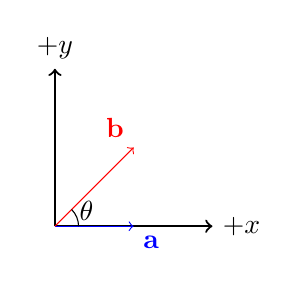
\begin{tikzpicture}
                \draw[->,thick] (0,0)--(2,0) node[right]{$+x$};
                \draw[->,thick] (0,0)--(0,2) node[above]{$+y$};
                \draw[->,blue] (0,0)--(1,0) node[anchor=north west]{$\mathbf{a}$};
                \draw[->,red] (0,0)--(1,1) node[anchor=south east]{$\mathbf{b}$};
                \draw (0.3,0) arc (0:45:0.3);
                \node at (0.4,0.2) {$\theta$};
            \end{tikzpicture}
            \hspace*{10pt}
            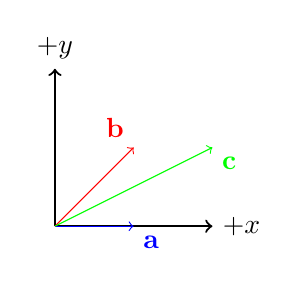
\begin{tikzpicture}
                \draw[->,thick] (0,0)--(2,0) node[right]{$+x$};
                \draw[->,thick] (0,0)--(0,2) node[above]{$+y$};
                \draw[->,blue] (0,0)--(1,0) node[anchor=north west]{$\mathbf{a}$};
                \draw[->,red] (0,0)--(1,1) node[anchor=south east]{$\mathbf{b}$};
                \draw[->,green] (0,0)--(2,1) node[anchor=north west]{$\mathbf{c}$};
            \end{tikzpicture}
        \end{center}

        For angles $0 < \theta < \pi / 2$ radians we can say $0 < \cos{(\theta) < 1}$. Letting $\alpha = 2||a||||b||\cos{(\theta)}$ this means we can say $\approx 2||a||||b|| < \alpha < 0$. Regardless 
        of the angle for $\theta$ we can say $\alpha > 0$. Intuitively, we can see that the length of the vector $c$ (defined as $a+b$) is greater than that of the sum of the two vectors $a$ and $b$'s 
        lengths. Mathematically this can be seen as

        \begin{equation}
            ||a + b|| > \sqrt{||a||^{2} + ||b||^{2}}.
        \end{equation}
        This of course only is possible if the angle between the vectors $a$ and $b$ is acute ($0 < \theta < \pi / 2$).
    \end{highlight}

    \begin{highlight}[Solution - Part (c)]
        For this problem I will be using \textbf{Method 4}. \vspace*{1em}

        We once again use equation (3.1) from VMLS in a new form 

        \begin{equation}
            ||a + b|| = \sqrt{||a||^{2} + 2||a||||b||\cos{(\theta)} + ||b||^2}.
        \end{equation}

        An angle $\theta$ is said to obtuse if $\pi / 2 < \theta < \pi$ radians. The image below shows an example of an obtuse angle and the superposition of the two vectors $a$ and $b$.

        \begin{center}
            \begin{tikzpicture}
                \draw[->,thick] (0,0)--(2,0) node[right]{$+x$};
                \draw[->,dotted] (0,0)--(-2,0) node[left]{$-x$};
                \draw[->,thick] (0,0)--(0,2) node[above]{$+y$};
                \draw[->,dotted] (0,0)--(0,-2) node[below]{$-y$};
                \draw[->,blue] (0,0)--(1,0) node[anchor=north west]{$\mathbf{a}$};
                \draw[->,red] (0,0)--(-1,1) node[anchor=south east]{$\mathbf{b}$};
                \draw (0.3,0) arc (0:135:0.3);
                \node at (0.3,0.4) {$\theta$};
            \end{tikzpicture}
            \hspace*{10pt}
            \begin{tikzpicture}
                \draw[->,thick] (0,0)--(2,0) node[right]{$+x$};
                \draw[->,dotted] (0,0)--(-2,0) node[left]{$-x$};
                \draw[->,thick] (0,0)--(0,2) node[above]{$+y$};
                \draw[->,dotted] (0,0)--(0,-2) node[below]{$-y$};
                \draw[->,blue] (0,0)--(1,0) node[anchor=north west]{$\mathbf{a}$};
                \draw[->,red] (0,0)--(-1,1) node[anchor=south east]{$\mathbf{b}$};
                \draw[->,green] (0,0)--(0,1) node[above]{$\mathbf{c}$};
            \end{tikzpicture}
        \end{center}

        For angles $\pi / 2 < \theta < \pi$ radians we can say $-1 < \cos{(\theta) < 0}$. Letting $\alpha = 2||a||||b||\cos{(\theta)}$ this means we can say $\approx -2||a||||b|| < \alpha < 0$. Regardless 
        of the angle for $\theta$ we can say $\alpha < 0$. Intuitively, we can see that the length of the vector $c$ (defined as $a+b$) is less than that of the sum of the two vectors $a$ and $b$'s 
        lengths. Mathematically this can be seen as

        \begin{equation}
            ||a + b|| < \sqrt{||a||^{2} + ||b||^{2}}.
        \end{equation}
        This of course only is possible if the angle between the vectors $a$ and $b$ is obtuse ($\pi / 2 < \theta < \pi$).
    \end{highlight}
\end{problem}

% Problem 2 Summary
\begin{summary}{Problem 2 Summary}
    \begin{statement}{Procedure}
        \begin{enumerate}[label = (\alph*)]
            \item Part (a)
            \begin{itemize}
                \item Use the formula for the sum of norms and show that the middle term in the formula is zero when the two vectors are perpendicular ($\theta = \frac{n\pi}{2}$)
            \end{itemize}
            \item Part (b)
            \begin{itemize}
                \item Use the formula for the sum of norms and show that the middle term in the formula will evaluate to less than $2\|a\|\|b\|$ when the angle between the vectors is acute 
                ($\theta < \frac{\pi}{2}$)
                \item Show that $\|a + b\|$ is then greater than the right hand side of the expression
            \end{itemize}
            \item Part (c)
            \begin{itemize}
                \item Use the formula for the sum of norms and show that the middle term in the formula will evaluate to greater than $2\|a\|\|b\|$ when the angle between the vectors is obtuse
                ($\theta > \frac{\pi}{2}$)
                \item Show that $\|a + b\|$ is then less than the right hand side of the expression
            \end{itemize}
        \end{enumerate}
    \end{statement}
    \begin{statement}{Key Concepts}
        \begin{itemize}
            \item The formula for the norm of one vector is
            \begin{equation*}
                \|x\| = \sqrt{x_{1}^{2} + \dots + x_{n}^{2}}
            \end{equation*}
            and the formula for finding the norm of two vectors is            
            \begin{equation*}
                \|x + y\| = \sqrt{\|x\|^{2} + 2x^{T}y + \|y\|^{2}}.
            \end{equation*}
            \item When two vectors are perpendicular to one another, then we can say that the relationship between the sum of norms is then
            \begin{equation*}
                ||a+b|| = \sqrt{||a||^{2} + ||b||^{2}}.
            \end{equation*}
            \item When the angle between two vectors is acute, we can then say that the relationship between the sum of norms is then
            \begin{equation*}
                ||a + b|| > \sqrt{||a||^{2} + ||b||^{2}}.
            \end{equation*}
            \item When the angle between two vectors is obtuse, we can then say that the relationship between the sum of norms is then
            \begin{equation*}
                ||a + b|| < \sqrt{||a||^{2} + ||b||^{2}}.
            \end{equation*}
        \end{itemize}
    \end{statement}
    \begin{statement}{Variations}
        \begin{itemize}
            \item The only way that this problem could be changed is if the expression that we are trying to prove is different
            \begin{itemize}
                \item We would then have to use the same procedure in evaluating different values of $\theta$ and whatnot for the expression
            \end{itemize}
        \end{itemize}
    \end{statement}
\end{summary}

% Problem 3
\begin{problem}{Problem 3}
    \begin{statement}{Problem Statement}
        Explain the solution to 3.1 here in your own words. (Since you are given a solution, you will be graded on your ability to explain). \vspace*{1em}

        \textbf{Original Question} \vspace*{1em}

        \textit{Distance between Boolean vectors}. Suppose that $x$ and $y$ are Boolean $n$-vectors, which means that each of their entries is either 0 or 1. What is their distance $||x-y||$?
    \end{statement}

    \begin{highlight}[Solution]
        For this problem I will be using \textbf{Method 4}. \vspace*{1em}

        \textbf{VMLS Solution:} \vspace*{1em}

        For each $i$, $x_{i}-y_{i}$ is either $-1,0,$ or $1$; $(x_{i}-y_{i})^{2}$ is zero (if $x_{i} = y_{i}$) or $1$ (if $x_{i} \neq y_{i}$). Summing over $i$, we find that $||x-y||^{2}$ is the total
        number of entries in which $x$ and $y$ differ. The distance is then the square root of the number of entries in which $x$ and $y$ differ. \vspace*{1em}

        \textbf{Explanation:} \vspace*{1em}

        Given two vectors $x$ and $y$ we know that there are a limited number of possibilities for the vectors in this scenario. Because of this we know the values of $x_{i} - y_{i}$ can only be

        \setcounter{equation}{0}
        \begin{align}
            x_{i} - y_{i} & = -1 & \text{(Lowest value. Occurs when $x_{i} = 0$ and $y_{i} = 1$)} \\
            & = 0 & \text{(Median value. Occurs when $x_{i} = y_{i}$)} \\
            & = 1 & \text{(Highest value. Occurs when $x_{i} = 1$ and $y_{i} = 0$)}.
        \end{align}
        This means for each element the only possible values for $(x_{i} - y_{i})^{2}$ are 

        \begin{align}
            (x_{i} - y_{i})^{2} & = 0 & \text{(Lowest value. Occurs when $x_{i}=y_{i}$)} \\
            & = 1 & \text{(Highest value. Occurs when $x_{i} \neq y_{i}$)}.
        \end{align}
        Regardless of the value of $x_{i} - y_{i}$ in equations (1)-(3), the distance between these boolean vectors is then 

        \begin{equation}
            ||x - y|| = \sqrt{\sum^{n}_{i = 1}(x_{i} - y_{i})^{2}}.
        \end{equation}
        Where $i$ is the index of the given element of a vector and $n$ is the length of the vectors.
    \end{highlight}
\end{problem}

% Problem 3 Summary
\begin{summary}{Problem 3 Summary}
    \begin{statement}{Procedure}
        \begin{itemize}
            \item Determine what the possible values of the entries can be between the two entries of the vectors
            \item Determine what the distance between the entries can be for the given values
        \end{itemize}
    \end{statement}
    \begin{statement}{Key Concepts}
        \begin{itemize}
            \item Boolean vectors are vectors where the entries are either a 0 or 1
            \item The distance between two vectors is calculated with 
            \begin{equation*}
                \mathbf{dist}(a,b) = \|a - b\|
            \end{equation*}
            \item The distance between entries of boolean vectors can either be 0 or 1
        \end{itemize}
    \end{statement}
    \begin{statement}{Variations}
        \begin{itemize}
            \item We could be given a different vector to determine what the distance between these entries would be
            \begin{itemize}
                \item In this case we would have to determine the possible values of each entry and then what the possible distance between those entries would be
            \end{itemize}
        \end{itemize}
    \end{statement}
\end{summary}

% Problem 4
\begin{problem}{Problem 4}
    \begin{statement}{Problem Statement}
        Explain the solution to 3.2 here in your own words. (Since you are given a solution, you will be graded on your ability to explain). \vspace*{1em}

        \textbf{Original Question} \vspace*{1em}

        \textit{RMS value and average of block vectors}. Let $x$ be a block vector with two vector elements, $x = (a,b)$, where $a$ and $b$ are vectors of size $n$ and $m$, respectively.

        \begin{enumerate}[label=(\alph*)]
            \item Express \textbf{rms}($x$) in terms of \textbf{rms}($a$), \textbf{rms}($b$), $m$, and $n$.
            \item Express \textbf{avg} in terms of \textbf{avg}($a$), \textbf{avg}($b$), $m$, and $n$.
        \end{enumerate}
    \end{statement}

    \begin{highlight}[Solution - Part (a)]
        For this problem I will be using \textbf{Method 4}. \vspace*{1em}

        \textbf{VMLS Solution:}

        \begin{enumerate}[label=(\alph*)]
            \item The RMS value of the vector $x = (a_{1}, \dots, a_{n}, b_{1}, \dots, b_{m})$ is 
            \begin{align*}
                \mathbf{rms}(x) & = \Bigg(\frac{a^{2}_{1} + \dots + a^{2}_{n} + b^{2}_{1} + \dots + b^{2}_{m}}{n + m}\Bigg)^{1/2} \\
                & = \Bigg(\frac{n(a^{2}_{1} + \dots + a^{2}_{n})/n + m(b^{2}_{1} + \dots + b^{2}_{m})/m}{n+m} \Bigg)^{1/2} \\
                & = \Bigg(\frac{n\mathbf{rms}(a)^{2} + m\mathbf{rms}(b)^{2}}{n+m} \Bigg)^{1/2}.
            \end{align*}
        \end{enumerate}

        \textbf{Explanation:} \vspace*{1em}

        In its simplest terms, the root mean square of a vector $\mu$ can be defined as 

        \setcounter{equation}{0}
        \begin{equation}
            \mathbf{rms}(\mu) = \sqrt{\frac{\mu^{2}_{1} + \dots + \mu^{2}_{\alpha}}{\alpha}} = \frac{||\mu||}{\sqrt{\alpha}}.
        \end{equation}
        The vector $x$ that was given to us in the problem statement is a concatenated vector of two vectors $a$ and $b$ where the length of $x$ is defined as $\alpha$. Concisely, we can rewrite $\alpha$
        as 

        \begin{equation}
            \alpha = n + m
        \end{equation}
        where $n$ is the vector length of $a$ and $m$ is the vector length of $b$. This means, if we re-write equation (1) for that of vector $x$ we will have

        \begin{equation}
            \mathbf{rms}(x) = \sqrt{\frac{x^{2}_{1} + \dots + x^{2}_{\alpha}}{\alpha}} = \Bigg(\frac{a^{2}_{1} + \dots + a^{2}_{n} + b^{2}_{1} + \dots + b^{2}_{m}}{n + m} \Bigg)^{1/2}
        \end{equation}
        where we have used the definition of an inner product for a concatenated vector in the numerator of equation (3). To get equation (3) written in terms of the \textbf{rms} of both sub vectors $a$ and
        $b$ we first need to \textit{sneakily} multiply by 1 for both the inner product of $a$ and $b$ in the numerator of equation (3). Applying a completeness relation to the inner products of both vectors $a$
        and $b$ in equation (3) we now have

        \begin{equation}
            \mathbf{rms}(x) = \Bigg(\frac{n(a^{2}_{1} + \dots + a^{2}_{n})/n + m(b^{2}_{1} + \dots + b^{2}_{m})/m}{n + m} \Bigg)^{1/2}
        \end{equation}
        where all we have done to equation (3) is multiplying by a constant value of 1 to both the inner products of $a$ and $b$ with the lengths of their vectors respectively. Observing equation (4) more closely
        we can see that we can right the square of the \textbf{rms} of a vector generically as

        \begin{equation}
            \mathbf{rms}^{2}(\mu) = \frac{\mu^{2}_{1} + \dots + \mu^{2}_{\alpha}}{\alpha}.
        \end{equation}
        Applying equation (5) to both vectors $a$ and $b$ in equation (3) we have the \textbf{rms}($x$) in terms of the \textbf{rms}($a$) and \textbf{rms}($b$) to be

        \begin{equation}
            \mathbf{rms}(x) = \Bigg(\frac{n\mathbf{rms}(a)^{2} + m\mathbf{rms}(b)^{2}}{n+m} \Bigg)^{1/2}.
        \end{equation}
        Equation (6) represents the \textbf{rms}($x$) in terms of the \textbf{rms} of both sub vectors $a$ and $b$.
    \end{highlight}

    \begin{highlight}[Solution - Part (b)]
        For this problem I will be using \textbf{Method 4}. \vspace*{1em}

        \textbf{VMLS Solution:}

        \begin{enumerate}[label=(\alph*), start=2]
            \item The average of the vector $x = (a_{1}, \dots, a_{n}, b_{1}, \dots, b_{m})$ is
            \begin{equation*}
                \mathbf{avg}(x) = \frac{a_{1} + \dots + a_{n} + b_{1} + \dots + b_{m}}{n + m} = \frac{n\mathbf{avg}(a) + m\mathbf{avg}(b)}{n + m}.
            \end{equation*}
        \end{enumerate}

        \textbf{Explanation:} \vspace*{1em}

        We define \textbf{avg} of some arbitrary vector $\mu$ with length $\alpha$ to be 

        \begin{equation}
            \mathbf{avg}(\mu) = \frac{\mu_{1} + \dots + \mu_{\alpha}}{\alpha}.
        \end{equation}
        In the context of our concatenated vector $x$ that was given to us in the problem statement, the lengths of sub vectors $a$ and $b$ are $n$ and $m$ respectively. This means the value of $\alpha$
        is the same as that of equation (2) from part (a). With this in mind, equation (7) now becomes 

        \begin{equation}
            \mathbf{avg}(x) = \frac{a_{1} + \dots + a_{n} + b_{1} + \dots + b_{m}}{n + m}
        \end{equation}
        for vector $x$ with sub vectors $a$ and $b$. Similar to part (a), we now apply a completeness relation to both vectors $a$ and $b$ found in equation (8) with the lengths of each respective vector
        to get

        \begin{equation}
            \mathbf{avg}(x) = \frac{n(a_{1} + \dots + a_{n})/n + m(b_{1} + \dots + b_{m})/m}{n + m}.
        \end{equation}
        Utilizing the generic definition for the average of a vector in equation (7) we can re-write equation (9) to now be in terms of the averages of both $a$ and $b$. Namely,

        \begin{equation}
            \mathbf{avg}(x) = \frac{n\mathbf{avg}(a) + m\mathbf{avg}(b)}{n + m}
        \end{equation}
        where equation (10) is the desired result that we have been working towards.
    \end{highlight}
\end{problem}

% Problem 4 Summary
\begin{summary}{Problem 4 Summary}
    \begin{statement}{Procedure}
        \begin{enumerate}[label = (\alph*)]
            \item Part (a)
            \begin{itemize}
                \item Use the general form of \textbf{rms} for one vector and apply it to both vectors
                \item Put this form into the expression
                \item Manipulate this form so that it can match the form of that is requested of us by multiplying by 1
                \item Simplify this form so that it is written in terms of \textbf{rms}
            \end{itemize}
            \item Part (b)
            \begin{itemize}
                \item Use the same process as in part (a) with \textbf{avg} instead of \textbf{rms}
            \end{itemize}
        \end{enumerate}
    \end{statement}
    \begin{statement}{Key Concepts}
        \begin{itemize}
            \item We can write the \textbf{rms} and \textbf{avg} for concatenated vectors in the form of the respective values for each independent vector
            \item \textbf{rms} of a vector is calculated with 
            \begin{equation*}
                \mathbf{rms}(x) = \frac{\|x\|}{\sqrt{n}}
            \end{equation*}
            \item \textbf{avg} of a vector is calculated with
            \begin{equation*}
                \mathbf{avg}(x) = \frac{x_{1} + \dots + x_{n}}{n}
            \end{equation*}
        \end{itemize}
    \end{statement}
    \begin{statement}{Variations}
        \begin{itemize}
            \item We could be asked to write a different expression for a concatenated vector in the form of values for independent vectors
            \begin{itemize}
                \item In this case we would have to use the definition of whatever we are trying to write and then apply it to each individual vector
            \end{itemize}
        \end{itemize}
    \end{statement}
\end{summary}

% Problem 5
\begin{problem}{Problem 5}
    \begin{statement}{Problem Statement}
        Explain the solution to 3.4 here in your own words. (Since you are given a solution, you will be graded on your ability to explain). \vspace*{1em}

        \textbf{Original Question} \vspace*{1em}

        \textit{Norm identities}. Verify that the following identities hold for any two vectors $a$ and $b$ of the same size.

        \begin{enumerate}[label=(\alph*)]
            \item $(a+b)^{T}(a-b) = ||a||^{2} - ||b||^{2}$.
            \item $||a+b||^{2} + ||a-b||^{2} = 2(||a||^{2}+||b||^{2})$. This is called the \textit{parallelogram law}.
        \end{enumerate}
    \end{statement}

    \begin{highlight}[Solution - Part (a)]
        For this problem I will be using \textbf{Method 4}. \vspace*{1em}

        \textbf{VMLS Solution:}

        \begin{enumerate}[label=(\alph*)]
            \item 
            \begin{align*}
                (a+b)^{T}(a-b) & = a^{T}(a-b) + b^{T}(a-b) \\
                & = a^{T}a - a^{T}b + b^{T}a - b^{T}b \\
                & = a^{T}a - a^{T}b + a^{T}b - b^{T}b \\
                & = a^{T}a - b^{T}b \\
                & = ||a||^{2} - ||b||^{2}
            \end{align*}
        \end{enumerate}

        \textbf{Explanation:} \vspace*{1em}

        To verify this identity, we have to take advantage of some properties pertaining to vectors as well as inner products of vectors. We first take advantage of the \textit{distributive} property
        of vector addition. Namely,

        \setcounter{equation}{0}
        \begin{equation}
            (a + b)^{T}c = a^{T}c + b^{T}c.
        \end{equation}
        We also have to use the \textit{commutative} property of inner products, namely

        \begin{equation}
            a^{T}b = b^{T}a.
        \end{equation}
        Using these properties we can go on to show

        \begin{align}
            (a+b)^{T}(a-b) & = a^{T}(a-b) + b^{T}(a-b) & \text{(Distributive property of inner products)} \\
            & = a^{T}a - a^{T}b + b^{T}a - b^{T}b & \text{(Distributive property of inner products)} \\
            & = a^{T}a - a^{T}b + a^{T}b - b^{T}b & \text{(Commutative property of inner products)} \\
            & = a^{T}a - b^{T}b & \text{(Simplification by addition)} \\
            & = ||a||^{2} - ||b||^{2} & \text{(Definition of inner product)}.
        \end{align}
        We have shown what was asked of us to show.
    \end{highlight}

    \begin{highlight}[Solution - Part (b)]
        For this problem I will be using \textbf{Method 4}. \vspace*{1em}

        \textbf{VMLS Solution:}

        \begin{enumerate}[label=(\alph*), start=2]
            \item 
            \begin{align*}
                ||a + b||^{2} + ||a - b||^{2} & = (a + b)^{T}(a + b) + (a - b)^{T}(a - b) \\
                & = a^{T}a + b^{T}a + a^{T}b + b^{T}b + a^{T}a - b^{T}a - a^{T}b + b^{T}b \\
                & = 2a^{T}a + 2b^{T}b \\
                & = 2||a||^{2} + 2||b||^{2}
            \end{align*}
        \end{enumerate}

        \textbf{Explanation:} \vspace*{1em}

        To verify this identity, we need to use the definition of norm. The norm of a vector is defined as

        \begin{equation}
            ||x|| = \sqrt{x^{2}_{1} + \dots + x^{2}_{n}}
        \end{equation}
        for a vector $x$ with length $n$. Extrapolating from equation (8) we can then say

        \begin{align}
            ||a + b||^{2} + ||a - b||^{2} & = (a + b)^{T}(a + b) + (a - b)^{T}(a - b) & \text{(Distributivity of norms)} \\
            & = a^{T}a + b^{T}a + a^{T}b + b^{T}b + a^{T}a - b^{T}a - a^{T}b + b^{T}b & \text{(Distributivity of norms)} \\
            & = a^{T}a + b^{T}b + a^{T}a + b^{T}b & \text{(Simplification by subtraction)} \\
            & = 2a^{T}a + 2b^{T}b & \text{(Simplification by addition)} \\
            & = 2||a||^{2} + 2||b||^{2} & \text{(Definition of inner products)}.
        \end{align}
        We have shown what was asked of us to show.
    \end{highlight}
\end{problem}

% Problem 5 Summary
\begin{summary}{Problem 5 Summary}
    \begin{statement}{Procedure}
        \begin{enumerate}[label = (\alph*)]
            \item Part (a)
            \begin{itemize}
                \item Apply the distributive property for transposes to the term $(a+b)^{T}(a-b)$
                \item Apply the commutative property for inner products 
                \item Simplify the terms and use the definition norm to reach the conclusion
            \end{itemize}
            \item Part (b)
            \begin{itemize}
                \item Apply the definition of norms to the term $||a+b||^{2} + ||a-b||^{2}$
                \item Use the distributive property of transposes and simplify terms in the following expressions
                \item Use the definition of inner products to simplify the final expression
            \end{itemize}
        \end{enumerate}
    \end{statement}
    \begin{statement}{Key Concepts}
        \begin{itemize}
            \item Distributivity applies to transposes
            \item Commutativity applies to inner products
            \item We use the definition of norm to simplify terms in the expression
            \item We can say the following expressions are true
            \begin{align*}
                (a+b)^{T}(a-b) & = ||a||^{2} - ||b||^{2} \\
                ||a+b||^{2} + ||a-b||^{2} & = 2(||a||^{2}+||b||^{2})
            \end{align*}
        \end{itemize}
    \end{statement}
    \begin{statement}{Variations}
        \begin{itemize}
            \item We could be given different expressions to prove
            \begin{itemize}
                \item In this case we would use the same properties and work through the algebra to prove the expression
            \end{itemize}
        \end{itemize}
    \end{statement}
\end{summary}

% Problem 6
\begin{problem}{Problem 6}
    \begin{statement}{Problem Statement}
        Explain the solution to 3.10 here in your own words. (Since you are given a solution, you will be graded on your ability to explain). \vspace*{1em}

        \textbf{Original Question} \vspace*{1em}

        \textit{Nearest neighbor document}. Consider the 5 Wikipedia pages in table 3.1 on page 51. What is the nearest neighbor of (the word count histogram vector of) `Veterans Day' among the others?
        Does the answer make sense?
    \end{statement}

    \begin{highlight}[Solution]
        For this problem I will be using \textbf{Method 4}. \vspace*{1em}

        \textbf{VMLS Solution:} \vspace*{1em}

        Its nearest neighbor is the histogram vector associated with ‘Memorial Day’. (We can see this by scanning the first row or column of table 3.1.) Yes, it makes sense — these two pages describe 
        holidays, whereas the others do not. \vspace*{1em}

        \textbf{Explanation:} \vspace*{1em}

        We define the nearest neighbor for a vector $x$ with a total of $m$ neighbors to be $z_{j}$. In mathematical form this is

        \setcounter{equation}{0}
        \begin{equation}
            ||x - z_{j}|| \leq ||x - z_{i}||, \hspace*{5pt} i = 1,\dots,m.
        \end{equation}
        Quantitatively, the distance between $x$ (Veteran's day) and it's neighbors ($z_{i}$) is a scalar value that represents the distance between the two respective vectors. For a neighbor to be considered
        vector $x$'s closest neighbor ($z_{j}$), the distance between the two vectors must be less than or equal to that of all the other individual neighbors. Upon observing table 3.1 on page 51, it is painstakingly
        obvious that the distance between Veteran's day and the other neighbors that is the smallest is \textbf{Memorial Day}. Mathematically this is

        \begin{equation}
            |x - z_{j}| = 0.095
        \end{equation}
        where $z_{j}$ is indeed Memorial Day. Verifying this mathematically we see

        \begin{align}
            |x - z_{\text{MD}}| & = 0.095 & \text{(Memorial Day)} \\
            |x - z_{\text{AA}}| & = 0.130 & \text{(Academy Awards)} \\
            |x - z_{\text{GGA}}| & = 0.153 & \text{(Golden Globe Awards)} \\
            |x - z_{\text{SB}}| & = 0.170 & \text{(Super Bowl)}
        \end{align}
        where when this is compared to the others we see

        \begin{align}
            |x - z_{\text{MD}}| = 0.095 & \leq |x - z_{\text{AA}}| = 0.130 \\
            |x - z_{\text{MD}}| = 0.095 & \leq |x - z_{\text{GGA}}| = 0.153 \\
            |x - z_{\text{MD}}| = 0.095 & \leq |x - z_{\text{SB}}| = 0.170.
        \end{align}
        and hence, we have shown that Veteran's Day closest neighbor is Memorial Day.
    \end{highlight}
\end{problem}

\begin{summary}{Problem 6 Summary}
    \begin{statement}{Procedure}
        \begin{itemize}
            \item Use the definition of nearest neighbor to determine what the nearest neighbor of a specific vector is
        \end{itemize}
    \end{statement}
    \begin{statement}{Key Concepts}
        \begin{itemize}
            \item Nearest neighbor is defined to be the vector that is the closest vector to another given vector
            \item The nearest neighbor $z_{j}$ to a vector $x$ with a total of $n$ vectors is 
            \begin{equation*}
                ||x - z_{j}|| \leq ||x - z_{i}||, \hspace*{5pt} i = 1,\dots,n
            \end{equation*}
        \end{itemize}
    \end{statement}
    \begin{statement}{Variations}
        \begin{itemize}
            \item We could be given a different data set to examine and determine what its nearest neighbor is
            \begin{itemize}
                \item In this case we would use the definition of nearest neighbor to determine what the nearest neighbor of a vector is
            \end{itemize}
        \end{itemize}
    \end{statement}
\end{summary}

% Problem 7
\begin{problem}{Problem 7}
    \begin{statement}{Problem Statement}
        Explain the solution to 3.20 here in your own words. (Since you are given a solution, you will be graded on your ability to explain). \vspace*{1em}

        \textbf{Original Question} \vspace*{1em}

        \textit{Regression model sensitivity}. Consider the regression model $\hat{y} = x^{T}x + v$, where $\hat{y}$ is the prediction, $x$ is a feature vector, $\beta$ is a coefficient vector, and
        $v$ is the offset term. If $x$ and $\tilde{x}$ are feature vectors with corresponding predictions $\hat{y}$ and $\tilde{y}$, show that $|\hat{y} - \tilde{y}| \leq ||\beta|| ||x - \tilde{x}||$.
        This means that when $||\beta||$ is small, the prediction is not very sensitive to a change in the feature vector.
    \end{statement}

    \begin{highlight}[Solution]
        For this problem I will be using \textbf{Method 4}. \vspace*{1em}

        \textbf{VMLS Solution:} \vspace*{1em}

        \textbf{Solution.} The inequality follows the Cauchy-Schwarz inequality:

        \begin{equation*}
            |\hat{y} - \tilde{y}| = |\beta^{T}x + v - (\beta^{T}\tilde{x} + v)| = |\beta^{T}(x - \tilde{x})| \leq ||\beta||||x - \tilde{x}||.
        \end{equation*}

        \textbf{Explanation:} \vspace*{1em}

        From the problem statement, we can say in general for this regression model

        \setcounter{equation}{0}
        \begin{equation}
            \alpha = \gamma^{T}\delta + v
        \end{equation}
        where $\alpha$ is the prediction, $\gamma$ is the coefficient vector, $\delta$ is the feature vector, and $v$ is the offset term. Using equation (1) we can extrapolate to say for this specific
        problem that

        \begin{align}
            \hat{y} & = \beta^{T}x + v \\
            \tilde{y} & = \beta^{T}\tilde{x} + v.
        \end{align}
        Taking the results from equations (2) and (3) we can then say 

        \begin{align}
            |\hat{y} - \tilde{y}| & = |\beta^{T}x + v - (\beta^{T}\tilde{x} + v)| & \text{(Substitution)} \\
            & = |\beta^{T}x + v - \beta^{T}\tilde{x} - v| & \text{(Distributivity)} \\
            & = |\beta^{T}x - \beta^{T}\tilde{x} + v - v| & \text{(Commutativity)} \\
            & = |\beta^{T}x - \beta^{T}\tilde{x}| & \text{(Simplification by subtraction)} \\
            & = |\beta^{T}(x - \tilde{x})| & \text{(Factoring)} \\
            & \leq ||\beta||||(x - \tilde{x})|| & \text{(Commutativity of norms)}.
        \end{align}
        Where equation (9) represents the desired inequality that we have been asked to show.
    \end{highlight}
\end{problem}

\begin{summary}{Problem 7 Summary}
    \begin{statement}{Procedure}
        \begin{itemize}
            \item Use the definition of the Cauchy Schwarz inequality and apply it to the two regression models
        \end{itemize}
    \end{statement}
    \begin{statement}{Key Concepts}
        \begin{itemize}
            \item A regression model is of the form
            \begin{equation*}
                \alpha = \gamma^{T}\delta + v
            \end{equation*}
            \item The Cauch Schwarz inequality is
            \begin{equation*}
                \|a^{T}b\| \leq \|a\|\|b\|
            \end{equation*}
            \item It can be shown that for two regression models the Cauchy Schwarz inequality is 
            \begin{equation*}
                |\hat{y} - \tilde{y}| \leq ||\beta||||(x - \tilde{x})||
            \end{equation*}
        \end{itemize}
    \end{statement}
    \begin{statement}{Variations}
        \begin{itemize}
            \item We could be asked to prove a different relationship
            \begin{itemize}
                \item We would then use the same properties and definitions just with a different premise
            \end{itemize}
        \end{itemize}
    \end{statement}
\end{summary}

% Problem 8
\begin{problem}{Problem 8}
    \begin{statement}{Problem Statement}
        Explain the solution to 3.23 here in your own words. (Since you are given a solution, you will be graded on your ability to explain). \vspace*{1em}

        \textbf{Original Question} \vspace*{1em}

        \textit{Angle between two nonnegative vectors}. Let $x$ and $y$ be two nonzero $n$-vectors with nonnegative entries, i.e., each $x_{i} \geq 0$ and each $y_{i} \geq 0$. Show that the angle between
        $x$ and $y$ lies between 0 and 90$^{\circ}$. Draw a picture for the case when $n = 2$, and give a short geometric explanation. When are $x$ and $y$ orthogonal?
    \end{statement}

    \begin{highlight}[Solution]
        For this problem I will be using \textbf{Method 4}. \vspace*{1em}

        \textbf{VMLS Solution:} \vspace*{1em}

        The angle lies between 0 and $90^{\circ}$ because the inner product of two elementwise nonnegative vectors, which is a sum of products of nonnegative numbers, is nonnegative. When $n = 2$, the two 
        vectors lie in the positive orthant, also known as quadrant I. The maximum angle between any such vectors is clearly $90^{\circ}$. This is illustrated below.

        \begin{center}
            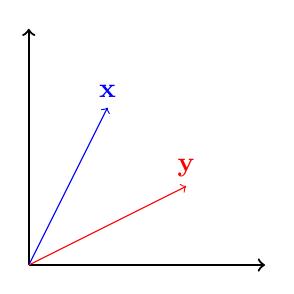
\begin{tikzpicture}
                \draw[->,thick] (0,0)--(3,0);
                \draw[->,thick] (0,0)--(0,3);
                \draw[->,blue] (0,0)--(1,2) node[anchor=south]{$\mathbf{x}$};
                \draw[->,red] (0,0)--(2,1) node[anchor=south]{$\mathbf{y}$};
            \end{tikzpicture}
        \end{center}
        Two nonnegative vectors are orthogonal if and only if they have a complementary zero-nonzero pattern, i.e., $x_{k} = 0$ whenever $y_{k} > 0$ and $y_{k} = 0$ whenever $x_{k} > 0$. \vspace*{1em}

        \textbf{Explanation:} \vspace*{1em}

        Mathematically, the inner product between two vectors $x$ and $y$ can be defined as

        \setcounter{equation}{0}
        \begin{equation}
            x^{T}y = ||x||||y||\cos{(\theta)}
        \end{equation}
        where $\theta$ is defined as the angle between two vectors. Solving for the angle $\theta$ in equation (1) yields 

        \begin{equation}
            \theta = \arccos{\Bigg(\frac{x^{T}y}{||x||||y||}\Bigg)}.
        \end{equation}
        In equation (2), it is a condition of trigonometric functions that the numerator found in $\arccos$ must be less than that of the denominator. Because the quantities $x^{T}y$ and $||x||$ as 
        well as $||y||$ are positive values for vectors with nonnegative entries, this constitutes that the value that is computed for $\arccos$ must be

        \begin{equation}
            0 \leq \arccos{\Bigg(\frac{x^{T}y}{||x||||y||}\Bigg)} \leq \pi / 2 \hspace*{10pt} , \hspace*{10pt} 0 \leq \theta \leq \pi / 2.
        \end{equation}
        The vectors will be orthogonal when the inner product between the two vectors is 0, or in terms of angles, when the angle between the vectors is $\pi / 2$. Because of the minimum and maximum angle 
        $\theta$ is either 0 or $\pi / 2$, we can confidently say that these vectors will lie in the \textbf{first quadrant}. These vectors could resemble something like what is illustrated below.

        \begin{center}
            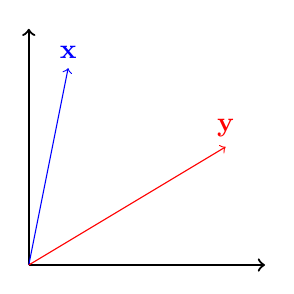
\begin{tikzpicture}
                \draw[->,thick] (0,0)--(3,0);
                \draw[->,thick] (0,0)--(0,3);
                \draw[->,blue] (0,0)--(0.5,2.5) node[anchor=south]{$\mathbf{x}$};
                \draw[->,red] (0,0)--(2.5,1.5) node[anchor=south]{$\mathbf{y}$};
            \end{tikzpicture}
            \hspace*{50pt}
            \begin{tikzpicture}
                \draw[->,thick] (0,0)--(3,0);
                \draw[->,thick] (0,0)--(0,3);
                \draw[->,blue] (0,0)--(0,2.5) node[anchor=south west]{$\mathbf{x}$};
                \draw[->,red] (0,0)--(2.5,0) node[anchor=south east]{$\mathbf{y}$};
            \end{tikzpicture}
            \hspace*{50pt}
            \begin{tikzpicture}
                \draw[->,thick] (0,0)--(3,0);
                \draw[->,thick] (0,0)--(0,3);
                \draw[->,blue] (0,0)--(0,2.5) node[anchor=south west]{$\mathbf{x}$};
                \draw[->,red] (0,0)--(0,1.5) node[anchor=south east]{$\mathbf{y}$};
            \end{tikzpicture}
        \end{center}
        The image that is furthest to the left is an example of two vectors where the angle between them is greater than 0 and less than $\pi / 2$. The middle image is an example of two vectors where 
        two vectors are orthogonal (perpendicular) where the angle between them is $\pi / 2$. The image that is furthest to the right is an example where the vectors are parallel to one another and 
        the angle between them is 0.
    \end{highlight}
\end{problem}

% Problem 8 Summary
\begin{summary}{Problem 8 Summary}
    \begin{statement}{Procedure}
        \begin{itemize}
            \item Use the definition of inner product and solve it for the angle between the vectors
            \item Show what the vectors will look like for given values of $\theta$
        \end{itemize}
    \end{statement}
    \begin{statement}{Key Concepts}
        \begin{itemize}
            \item When vectors are orthogonal, the inner product of the two vectors is zero and the angle between them is $\pi / 2$
            \item When vectors are parallel, the inner product is non zero and the angle between them is less than $\pi / 2$
            \item When vectors are not orthogonal and parallel, then the angle between them is not 0 or $\pi / 2$
        \end{itemize}
    \end{statement}
    \begin{statement}{Variations}
        \begin{itemize}
            \item We could be given a different set of orientations for vectors
            \begin{itemize}
                \item We would have to figure out the angle between the vectors for this new orientation
            \end{itemize}
        \end{itemize}
    \end{statement}
\end{summary}

% Problem 9
\begin{problem}{Problem 9}
    \begin{statement}{Problem Statement}
        Explain the solution to 3.24 here in your own words. (Since you are given a solution, you will be graded on your ability to explain). Create your own example for part (a). \vspace*{1em}

        \textbf{Original Question} \vspace*{1em}

        \textit{Distance versus angle nearest neighbor}. Suppose $z_{1} , \dots , z_{m}$ is a collection of $n$-vectors, and $x$ is another $n$-vector. The vector $z_{j}$ is the (distance) nearest neighbor of
        $x$ (among the given vectors) if

        \begin{equation*}
            ||x-z_{j}|| \leq ||x - z_{i}||, \hspace*{5pt} i = 1 , \dots , m,
        \end{equation*}

        i.e., $x$ has smallest distance to $z_{j}$. We say that $z_{j}$ is the \textit{angle nearest neighbor} of $x$ if

        \begin{equation*}
            \angle (x,z_{j}) \leq \angle (x,z_{i}), \hspace*{5pt} i = 1 , \dots , m,
        \end{equation*}

        i.e., $x$ has smallest angle to $z_{j}$.

        \begin{enumerate}[label=(\alph*)]
            \item Give a simple specific numerical example where the (distance) nearest neighbor is not the same as the angle nearest neighbor.
            \item Now suppose that the vectors $z_{1} , \dots , z_{m}$ are normalized, which means that $||z_{i}||$, $i = 1 , \dots , m$. Show that in this case the distance nearest neighbor and the angle nearest 
            neighbor are always the same. \textit{Hint}. You can use the fact that arccos is a decreasing function, i.e., for any $u$ and $v$ with $-1 \leq u < v \leq 1$, we have $\arccos{(u)} > \arccos{(v)}$.
        \end{enumerate}
    \end{statement}

    \begin{highlight}[Solution - Part (a)]
        For this problem I will be using \textbf{Method 4}. \vspace*{1em}

        For this example, we will choose $n = 1$. We then choose $z_{1} = 2, z_{2} = -5$, and $x = 4$. We then have the results

        \setcounter{equation}{0}
        \begin{equation}
            ||x - z_{1}|| = 2 \hspace*{5pt} , \hspace*{5pt} ||x - z_{2}|| = 9 \hspace*{5pt} , \hspace*{5pt} \angle(x,z_{1}) \hspace*{5pt} , \hspace*{5pt} \angle(x,z_{2}) = 0.
        \end{equation}
        The nearest neighbor to $x$ is then $z_{2}$ and the angle nearest neighbor is $z_{2}$.
    \end{highlight}

    \begin{highlight}[Solution - Part (b)]
        For this problem I will be using \textbf{Method 4}. \vspace*{1em}

        To show what is asked of us, we do the following
        \horizontalline{0}{-2}
        \begin{align}
            \|x - z_j\| &\leq \|x - z_i\| \Leftrightarrow \|x - z_j\|^2 \leq \|x - z_i\|^2 & \text{(Premise)} \\
            &\Leftrightarrow \|x\|^2 - 2x^Tz_j + \|z_j\|^2 \leq \|x\|^2 - 2x^Tz_i + \|z_i\|^2 & \text{(Substitution)} \\
            &\Leftrightarrow -2x^Tz_j \leq -2x^Tz_i & \text{(Simplification by subtraction)} \\
            &\Leftrightarrow x^Tz_j \geq x^Tz_i & \text{(Simplification by division)} \\
            &\Leftrightarrow \frac{x^Tz_j}{\|x\|\|z_j\|} \geq \frac{x^Tz_i}{\|x\|\|z_i\|} & \text{($\cos{(\theta)}$ of inner products)} \\
            &\Leftrightarrow \arccos\left(\frac{x^Tz_j}{\|x\|\|z_j\|}\right) \leq \arccos\left(\frac{x^Tz_i}{\|x\|\|z_i\|}\right) & \text{($\theta$ of vectors)} \\
            &\Leftrightarrow \langle x, z_j \rangle \leq \langle x, z_i \rangle & \text{(Definition of inner product)}.
        \end{align}
        \horizontalline{-1}{0}
        Hence, the nearest neighbor and nearest neighbor angle will always be the same.   
    \end{highlight}
\end{problem}

% Problem 9 Summary
\begin{summary}{Problem 9 Summary}
    \begin{statement}{Procedure}
        \begin{enumerate}[label = (\alph*)]
            \item Part (a)
            \begin{itemize}
                \item Use the definition of nearest neighbor and evaluate what the nearest neighbor is for each entry
            \end{itemize}
            \item Part (b)
            \begin{itemize}
                \item Use definition of norm with the nearest neighbor definition and the appropriate properties to reach the conclusion
            \end{itemize}
        \end{enumerate}
    \end{statement}
    \begin{statement}{Key Concepts}
        \begin{itemize}
            \item We can find relationships between inner products and nearest neighbor
        \end{itemize}
    \end{statement}
    \begin{statement}{Variations}
        \begin{itemize}
            \item We could be given a different set of properties to prove
            \begin{itemize}
                \item We would then use the same properties and procedures to reach the conclusion
            \end{itemize}
        \end{itemize}
    \end{statement}
\end{summary}
\end{document}
%---------------------------------------------------------------------------
%	
%---------------------------------------------------------------------------